%!TEX root = ../../terrainbook.tex
% chktex-file 46

\graphicspath{{appendices/ahn/figs/}}

\chapter{Extra information about the AHN datasets}%
\label{app:ahn}


\begin{figure}
  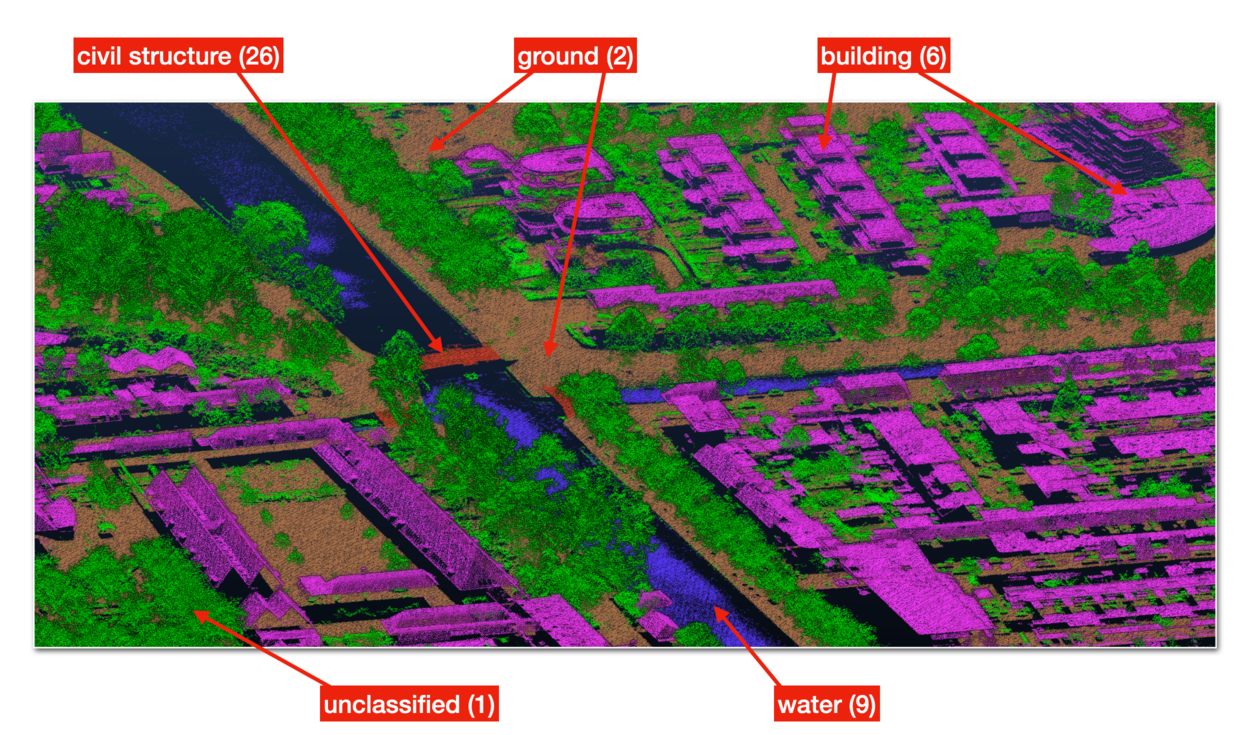
\includegraphics[width=\linewidth]{ahn4.png}
  \caption{Classification codes used in the AHN3+AHN4 datasets.}%
\label{fig:ahn3}
\end{figure}

The AHN dataset (\emph{Actueel Hoogtebestand Nederland} in Dutch, or ``actual height of the Netherlands''), 
\marginnote{\emph{Actueel Hoogtebestand Nederland} (AHN)}
\marginnote{\url{https://www.ahn.nl}}
is a lidar dataset that contains several points per $m^2$ and covers entirely the Netherlands.
It is an open dataset.

\marginnote{AHN5 is the current version}
It began in 1997, and its current version is 5 (called AHN5) (although it is not fully available online yet\sidenote{AHN5 status: \url{https://www.ahn.nl/tweede-deel-ahn5-beschikbaar}}.

The AHN5 dataset uses the ``Point Data Record Format 6'', see Table~\ref{tab:las-record}.

LAS v1.4 allows to store certain extra user-defined attributes, and in AHN4 the following 3 are also stored (but not in other versions):
\begin{enumerate}
  \item \emph{Amplitude:} echo signal amplitude [dB] (min: 0; max: 10000) 
  \item \emph{Reflectance:} echo signal reflectance [dB] (min: 0; max: 10000)
  \item \emph{Deviation:} pulse shape deviation (min: 0; max: 65535)
\end{enumerate}

%

The AHN lidar dataset is disseminated in the LAZ format (a compressed version of LAS, see Appendices~\ref{sec:lasformat} and~\ref{sec:lazformat}) and uses the LAS classification codes (see Table~\ref{tab:las-classes}). 
Figure~\ref{fig:ahn3} shows all the codes that are used. 
Notice that apart from the pre-defined codes from Table~\ref{tab:las-classes}, AHN4/5 also uses the custom code $26$ for a `civil structure' (Dutch: \emph{kunstwerk}) class that includes special infrastructures such as bridges, statues, and viaducts. 

%

It should be noticed that in AHN5 the class 6/\texttt{building} is for the roofs of the buildings \emph{only}, the façades of a building are in class 1/\texttt{unclassified}.
This is in contract to previous versions in which all points representing a building were classified as 6/\texttt{building}.

%

Observe also that in AHN the points representing vegetation are not classified as such, and vegetation is never explicitly classified.
\marginnote{vegetation is classified as $1$/\texttt{unclassified}}
The is because the aim of the AHN project is mostly to model dikes and to protect us from floods, and vegetation is not very important for this use-case.
The class $1$ is thus used for vegetation, but other objects such as street furniture (\eg\ lampposts) or cars are also classified as $1$.

%

Certain tiles contain the classification 14/\texttt{high-voltage pylons and cables}, but not all of them. 
\marginnote{class=14 for pylons+cables (for some tiles only)}
If 14 is not used, the pylons and cables are in class 26/\texttt{kunstwerk}.

%


